\documentclass[tikz,crop,convert={density=200,outext=.png},border=0.4cm]{standalone}

\usepackage{pgfplots}
\usepackage{amsmath}
\usetikzlibrary{arrows.meta}
\usepackage{physics}
\usepackage{xcolor}
% Allee effect
\definecolor{clr_1}{RGB}{0,68,27}
% Generalised growth model
\definecolor{clr_2}{RGB}{2,56,88}
\pgfplotsset{compat=newest,
    %width=6cm,
    %height=3cm,
    scale only axis=true,
    max space between ticks=25pt,
    try min ticks=5,
    every axis/.style={
        axis y line=middle,
        axis x line=middle,
        axis line style={thick,->,>=latex, shorten >=-.3cm}
    },
    every axis plot/.append style={thick},
    tick style={black, thick},
}
\tikzset{
    semithick/.style={line width=0.8pt},
}
\usepgfplotslibrary{groupplots}
\usepgfplotslibrary{dateplot}
% Document begins
\begin{document}

% =========================================================================================================
% r trans figure stable node
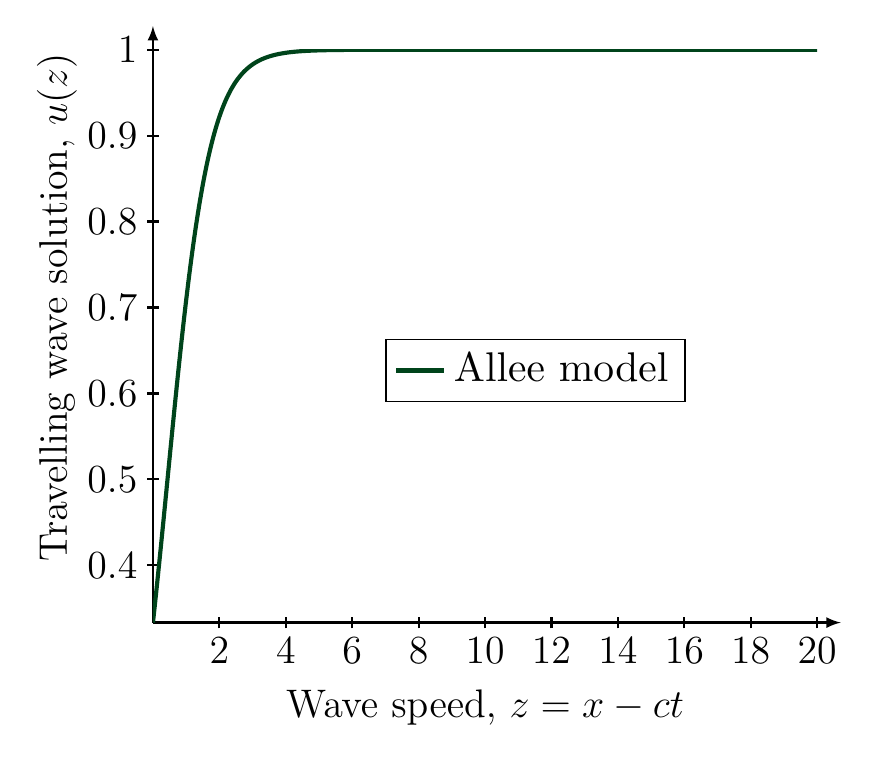
\begin{tikzpicture}
  % The axis of the plot
\begin{axis}[
    xlabel={Wave speed, $z=x-ct$},
    ylabel={Travelling wave solution, $u(z)$},
    x label style={at={(axis description cs:0.5,-0.1)},anchor=north},
    y label style={at={(axis description cs:-0.1,0.55)},rotate=90,anchor=south},
    %scaled x ticks = false,
    %xtick={-1,-0.5,...,2},
    % ymax = 4.5,
    %xmax = 4.5,
    legend style={at={(axis description cs:0.35,0.44)},anchor=west,nodes={scale=1.5, transform shape}},
    label style={font=\Large},
    tick label style={font=\Large},
    legend cell align={left},
    grid style=dashed,
]
\addplot[
color=clr_1,line width=1.5pt,
]
coordinates {%
(0.0,0.3333333333333333)
(0.04008016032064128,0.34756158420983513)
(0.08016032064128256,0.36206732327687147)
(0.12024048096192384,0.37682880477396663)
(0.16032064128256512,0.3918224665584488)
(0.2004008016032064,0.40702305453259996)
(0.24048096192384769,0.422403772254666)
(0.280561122244489,0.43793645425835515)
(0.32064128256513025,0.4535917610008096)
(0.3607214428857715,0.46933939278675413)
(0.4008016032064128,0.48514831949912013)
(0.4408817635270541,0.5009870225250717)
(0.48096192384769537,0.5168237449196084)
(0.5210420841683366,0.5326267456117223)
(0.561122244488978,0.5483645533408259)
(0.6012024048096192,0.564006216019005)
(0.6412825651302605,0.5795215413472565)
(0.6813627254509018,0.5948813247653767)
(0.721442885771543,0.6100575611746141)
(0.7615230460921844,0.6250236373241176)
(0.8016032064128256,0.6397545022776518)
(0.8416833667334669,0.6542268139546011)
(0.8817635270541082,0.6684190603463702)
(0.9218436873747494,0.682311654623297)
(0.9619238476953907,0.6958870039466888)
(1.002004008016032,0.7091295523662431)
(1.0420841683366733,0.7220257986984867)
(1.0821643286573146,0.7345642907339861)
(1.122244488977956,0.7467355975006941)
(1.1623246492985972,0.7585322616124305)
(1.2024048096192383,0.7699487339533071)
(1.2424849699398797,0.7809812930923231)
(1.282565130260521,0.7916279518916094)
(1.3226452905811623,0.801888353773372)
(1.3627254509018036,0.811763661052601)
(1.4028056112224447,0.8212564376342808)
(1.442885771543086,0.8303705282248515)
(1.4829659318637274,0.8391109360277789)
(1.5230460921843687,0.8474837006916428)
(1.56312625250501,0.8554957780647816)
(1.6032064128256511,0.8631549230909985)
(1.6432865731462925,0.8704695769627528)
(1.6833667334669338,0.8774487594371656)
(1.723446893787575,0.8841019670204273)
(1.7635270541082164,0.8904390775410579)
(1.8036072144288577,0.896470261464227)
(1.8436873747494988,0.9022059001493092)
(1.8837675350701402,0.9076565111216434)
(1.9238476953907815,0.9128326803169987)
(1.9639278557114228,0.9177450011629422)
(2.004008016032064,0.9224040202841914)
(2.0440881763527052,0.9268201895578482)
(2.0841683366733466,0.9310038241977102)
(2.124248496993988,0.9349650665131007)
(2.164328657314629,0.9387138549652548)
(2.2044088176352705,0.9422598981317084)
(2.244488977955912,0.9456126531848416)
(2.284569138276553,0.9487813084933342)
(2.3246492985971945,0.95177476996351)
(2.3647294589178354,0.9546016507501945)
(2.4048096192384767,0.9572702639827723)
(2.444889779559118,0.959788618170667)
(2.4849699398797593,0.9621644149727353)
(2.5250501002004007,0.9644050490363572)
(2.565130260521042,0.9665176096338018)
(2.6052104208416833,0.9685088838452794)
(2.6452905811623246,0.9703853610595846)
(2.685370741482966,0.9721532385841314)
(2.7254509018036073,0.9738184281762315)
(2.7655310621242486,0.9753865633265363)
(2.8056112224448895,0.9768630071435307)
(2.845691382765531,0.978252860704772)
(2.885771543086172,0.9795609717561666)
(2.9258517034068134,0.980791943654981)
(2.9659318637274548,0.9819501444654876)
(3.006012024048096,0.9830397161282063)
(3.0460921843687374,0.9840645836346381)
(3.0861723446893787,0.9850284641492776)
(3.12625250501002,0.9859348760295789)
(3.1663326653306614,0.9867871477025075)
(3.2064128256513023,0.9875884263634038)
(3.2464929859719436,0.9883416864691711)
(3.286573146292585,0.9890497380033655)
(3.3266533066132262,0.9897152344956449)
(3.3667334669338675,0.9903406807823135)
(3.406813627254509,0.9909284404984167)
(3.44689378757515,0.9914807432950706)
(3.4869739478957915,0.9919996917784806)
(3.527054108216433,0.9924872681694785)
(3.567134268537074,0.9929453406844302)
(3.6072144288577155,0.9933756696400567)
(3.6472945891783564,0.993779913286136)
(3.6873747494989977,0.9941596333712199)
(3.727454909819639,0.9945163004474532)
(3.7675350701402803,0.9948512989213424)
(3.8076152304609217,0.9951659318579185)
(3.847695390781563,0.9954614255461832)
(3.8877755511022043,0.995738933834062)
(3.9278557114228456,0.9959995422412938)
(3.967935871743487,0.9962442718588247)
(4.008016032064128,0.9964740830433116)
(4.04809619238477,0.9966898789153291)
(4.0881763527054105,0.9968925086697961)
(4.128256513026052,0.9970827707070202)
(4.168336673346693,0.9972614155926031)
(4.208416833667335,0.9974291488542546)
(4.248496993987976,0.9975866336233628)
(4.288577154308617,0.9977344931289241)
(4.328657314629258,0.997873313051203)
(4.368737474949899,0.9980036437422249)
(4.408817635270541,0.998126002319956)
(4.448897795591182,0.9982408746427444)
(4.488977955911824,0.9983487171703407)
(4.529058116232465,0.998449958717543)
(4.569138276553106,0.9985450021062485)
(4.609218436873747,0.9986342257214351)
(4.649298597194389,0.998717984976339)
(4.68937875751503,0.9987966136918461)
(4.729458917835671,0.9988704253948713)
(4.7695390781563125,0.9989397145402654)
(4.809619238476953,0.9990047576605631)
(4.849699398797595,0.9990658144476595)
(4.889779559118236,0.9991231287703023)
(4.929859719438878,0.9991769296310703)
(4.969939879759519,0.9992274320663276)
(5.01002004008016,0.9992748379924444)
(5.050100200400801,0.9993193370014067)
(5.090180360721443,0.9993611071087599)
(5.130260521042084,0.9994003154566748)
(5.170340681362725,0.999437118974766)
(5.210420841683367,0.9994716650011468)
(5.2505010020040075,0.9995040918660686)
(5.290581162324649,0.9995345294403525)
(5.33066132264529,0.9995630996507042)
(5.370741482965932,0.9995899169638779)
(5.410821643286573,0.9996150888415417)
(5.4509018036072145,0.9996387161675964)
(5.490981963927855,0.9996608936495897)
(5.531062124248497,0.9996817101957783)
(5.571142284569138,0.9997012492692994)
(5.611222444889779,0.9997195892208223)
(5.651302605210421,0.9997368036009784)
(5.691382765531062,0.9997529614537842)
(5.731462925851703,0.9997681275922051)
(5.771543086172344,0.9997823628569359)
(5.811623246492986,0.9997957243594139)
(5.851703406813627,0.9998082657100179)
(5.891783567134269,0.9998200372323486)
(5.9318637274549095,0.9998310861644357)
(5.971943887775551,0.9998414568476627)
(6.012024048096192,0.9998511909041566)
(6.052104208416833,0.9998603274033414)
(6.092184368737475,0.9998689030183151)
(6.132264529058116,0.9998769521726689)
(6.1723446893787575,0.9998845071783294)
(6.212424849699398,0.9998915983649722)
(6.25250501002004,0.9998982542015179)
(6.292585170340681,0.9999045014101952)
(6.332665330661323,0.9999103650736229)
(6.372745490981964,0.9999158687353381)
(6.4128256513026045,0.9999210344941688)
(6.452905811623246,0.9999258830928281)
(6.492985971943887,0.9999304340010826)
(6.533066132264529,0.9999347054938253)
(6.57314629258517,0.9999387147243672)
(6.613226452905812,0.9999424777932362)
(6.6533066132264524,0.9999460098127613)
(6.693386773547094,0.9999493249676976)
(6.733466933867735,0.9999524365721362)
(6.773547094188377,0.9999553571229239)
(6.813627254509018,0.9999580983498095)
(6.853707414829659,0.9999606712625142)
(6.8937875751503,0.9999630861949154)
(6.933867735470941,0.9999653528465222)
(6.973947895791583,0.999967480321406)
(7.014028056112224,0.9999694771647438)
(7.054108216432866,0.9999713513971195)
(7.0941883767535066,0.9999731105467216)
(7.134268537074148,0.9999747616795652)
(7.174348697394789,0.9999763114278603)
(7.214428857715431,0.9999777660166383)
(7.254509018036072,0.9999791312887475)
(7.294589178356713,0.9999804127283112)
(7.3346693386773545,0.9999816154827493)
(7.374749498997995,0.9999827443834471)
(7.414829659318637,0.9999838039651562)
(7.454909819639278,0.9999847984842043)
(7.49498997995992,0.9999857319355876)
(7.535070140280561,0.9999866080690148)
(7.575150300601202,0.9999874304039651)
(7.615230460921843,0.999988202243823)
(7.655310621242485,0.9999889266891452)
(7.695390781563126,0.9999896066501126)
(7.735470941883767,0.9999902448582192)
(7.775551102204409,0.9999908438772422)
(7.8156312625250495,0.9999914061135393)
(7.855711422845691,0.9999919338257138)
(7.895791583166332,0.9999924291336867)
(7.935871743486974,0.9999928940272107)
(7.975951903807615,0.9999933303738633)
(8.016032064128256,0.9999937399265477)
(8.056112224448897,0.9999941243305337)
(8.09619238476954,0.9999944851300667)
(8.13627254509018,0.9999948237745705)
(8.176352705410821,0.999995141624469)
(8.216432865731463,0.9999954399566517)
(8.256513026052104,0.999995719969602)
(8.296593186372744,0.999995982788212)
(8.336673346693386,0.9999962294683007)
(8.376753507014028,0.9999964610008558)
(8.41683366733467,0.9999966783160139)
(8.45691382765531,0.9999968822867973)
(8.496993987975952,0.9999970737326208)
(8.537074148296593,0.9999972534225834)
(8.577154308617233,0.9999974220785579)
(8.617234468937875,0.9999975803780907)
(8.657314629258517,0.9999977289571236)
(8.697394789579159,0.9999978684125485)
(8.737474949899799,0.999997999304605)
(8.77755511022044,0.9999981221591314)
(8.817635270541082,0.9999982374696768)
(8.857715430861724,0.9999983456994839)
(8.897795591182364,0.9999984472833496)
(8.937875751503006,0.9999985426293725)
(8.977955911823647,0.9999986321205915)
(9.018036072144287,0.9999987161165247)
(9.05811623246493,0.9999987949546141)
(9.098196392785571,0.9999988689515809)
(9.138276553106213,0.9999989384046979)
(9.178356713426853,0.9999990035929835)
(9.218436873747494,0.9999990647783233)
(9.258517034068136,0.9999991222065212)
(9.298597194388778,0.9999991761082876)
(9.338677354709418,0.9999992267001659)
(9.37875751503006,0.9999992741854026)
(9.418837675350701,0.9999993187547636)
(9.458917835671341,0.9999993605873008)
(9.498997995991983,0.9999993998510712)
(9.539078156312625,0.9999994367038123)
(9.579158316633267,0.9999994712935754)
(9.619238476953907,0.9999995037593207)
(9.659318637274549,0.9999995342314755)
(9.69939879759519,0.9999995628324579)
(9.739478957915832,0.9999995896771692)
(9.779559118236472,0.9999996148734547)
(9.819639278557114,0.9999996385225375)
(9.859719438877756,0.999999660719425)
(9.899799599198396,0.9999996815532909)
(9.939879759519037,0.9999997011078325)
(9.97995991983968,0.9999997194616081)
(10.02004008016032,0.9999997366883518)
(10.06012024048096,0.9999997528572703)
(10.100200400801603,0.9999997680333201)
(10.140280561122244,0.9999997822774694)
(10.180360721442886,0.9999997956469424)
(10.220440881763526,0.9999998081954495)
(10.260521042084168,0.999999819973403)
(10.30060120240481,0.9999998310281194)
(10.34068136272545,0.9999998414040098)
(10.380761523046091,0.9999998511427581)
(10.420841683366733,0.9999998602834888)
(10.460921843687375,0.9999998688629236)
(10.501002004008015,0.9999998769155296)
(10.541082164328657,0.9999998844736571)
(10.581162324649299,0.9999998915676702)
(10.62124248496994,0.9999998982260682)
(10.66132264529058,0.9999999044756005)
(10.701402805611222,0.9999999103413739)
(10.741482965931864,0.9999999158469535)
(10.781563126252504,0.9999999210144574)
(10.821643286573146,0.9999999258646455)
(10.861723446893787,0.9999999304170027)
(10.901803607214429,0.999999934689818)
(10.941883767535069,0.9999999387002566)
(10.98196392785571,0.9999999424644301)
(11.022044088176353,0.9999999459974608)
(11.062124248496994,0.999999949313542)
(11.102204408817634,0.9999999524259959)
(11.142284569138276,0.9999999553473264)
(11.182364729458918,0.9999999580892696)
(11.222444889779558,0.999999960662841)
(11.2625250501002,0.9999999630783796)
(11.302605210420841,0.9999999653455895)
(11.342685370741483,0.9999999674735791)
(11.382765531062123,0.9999999694708974)
(11.422845691382765,0.9999999713455683)
(11.462925851703407,0.999999973105123)
(11.503006012024048,0.9999999747566306)
(11.543086172344688,0.9999999763067255)
(11.58316633266533,0.9999999777616354)
(11.623246492985972,0.9999999791272051)
(11.663326653306612,0.9999999804089205)
(11.703406813627254,0.9999999816119308)
(11.743486973947896,0.999999982741069)
(11.783567134268537,0.9999999838008714)
(11.823647294589177,0.9999999847955956)
(11.863727454909819,0.9999999857292377)
(11.90380761523046,0.9999999866055485)
(11.943887775551103,0.9999999874280485)
(11.983967935871743,0.9999999882000421)
(12.024048096192384,0.9999999889246306)
(12.064128256513026,0.999999989604725)
(12.104208416833666,0.9999999902430576)
(12.144288577154308,0.9999999908421927)
(12.18436873747495,0.9999999914045372)
(12.224448897795591,0.9999999919323505)
(12.264529058116231,0.9999999924277527)
(12.304609218436873,0.9999999928927343)
(12.344689378757515,0.9999999933291633)
(12.384769539078157,0.9999999937387929)
(12.424849699398797,0.9999999941232688)
(12.464929859719438,0.9999999944841355)
(12.50501002004008,0.9999999948228429)
(12.54509018036072,0.9999999951407514)
(12.585170340681362,0.9999999954391386)
(12.625250501002004,0.999999995719203)
(12.665330661322646,0.9999999959820698)
(12.705410821643286,0.9999999962287949)
(12.745490981963927,0.9999999964603696)
(12.785571142284569,0.9999999966777242)
(12.825651302605209,0.999999996881732)
(12.86573146292585,0.9999999970732124)
(12.905811623246493,0.9999999972529349)
(12.945891783567134,0.9999999974216212)
(12.985971943887774,0.9999999975799492)
(13.026052104208416,0.999999997728555)
(13.066132264529058,0.9999999978680353)
(13.1062124248497,0.9999999979989508)
(13.14629258517034,0.9999999981218273)
(13.186372745490981,0.9999999982371585)
(13.226452905811623,0.9999999983454075)
(13.266533066132263,0.9999999984470095)
(13.306613226452905,0.9999999985423724)
(13.346693386773547,0.9999999986318796)
(13.386773547094188,0.9999999987158904)
(13.426853707414828,0.9999999987947424)
(13.46693386773547,0.9999999988687526)
(13.507014028056112,0.999999998938218)
(13.547094188376754,0.9999999990034177)
(13.587174348697394,0.9999999990646139)
(13.627254509018035,0.9999999991220523)
(13.667334669338677,0.9999999991759636)
(13.707414829659317,0.9999999992265644)
(13.747494989979959,0.999999999274058)
(13.7875751503006,0.9999999993186351)
(13.827655310621243,0.9999999993604751)
(13.867735470941883,0.9999999993997458)
(13.907815631262524,0.999999999436605)
(13.947895791583166,0.9999999994712009)
(13.987975951903808,0.9999999995036724)
(14.028056112224448,0.9999999995341499)
(14.06813627254509,0.9999999995627559)
(14.108216432865731,0.9999999995896053)
(14.148296593186371,0.999999999614806)
(14.188376753507013,0.9999999996384592)
(14.228456913827655,0.99999999966066)
(14.268537074148297,0.9999999996814976)
(14.308617234468937,0.9999999997010555)
(14.348697394789578,0.9999999997194124)
(14.38877755511022,0.9999999997366422)
(14.428857715430862,0.999999999752814)
(14.468937875751502,0.9999999997679927)
(14.509018036072144,0.9999999997822393)
(14.549098196392785,0.9999999997956112)
(14.589178356713425,0.9999999998081619)
(14.629258517034067,0.9999999998199419)
(14.669338677354709,0.9999999998309985)
(14.70941883767535,0.9999999998413762)
(14.74949899799599,0.9999999998511168)
(14.789579158316633,0.999999999860259)
(14.829659318637274,0.99999999986884)
(14.869739478957916,0.999999999876894)
(14.909819639278556,0.9999999998844534)
(14.949899799599198,0.9999999998915488)
(14.98997995991984,0.9999999998982083)
(15.03006012024048,0.9999999999044589)
(15.070140280561121,0.9999999999103257)
(15.110220440881763,0.9999999999158322)
(15.150300601202405,0.9999999999210006)
(15.190380761523045,0.9999999999258516)
(15.230460921843687,0.9999999999304048)
(15.270541082164328,0.9999999999346784)
(15.31062124248497,0.9999999999386895)
(15.35070140280561,0.9999999999424544)
(15.390781563126252,0.999999999945988)
(15.430861723446894,0.9999999999493047)
(15.470941883767534,0.9999999999524177)
(15.511022044088175,0.9999999999553395)
(15.551102204408817,0.999999999958082)
(15.591182364729459,0.9999999999606559)
(15.631262525050099,0.9999999999630719)
(15.67134268537074,0.9999999999653395)
(15.711422845691382,0.9999999999674679)
(15.751503006012024,0.9999999999694655)
(15.791583166332664,0.9999999999713406)
(15.831663326653306,0.9999999999731004)
(15.871743486973948,0.9999999999747522)
(15.911823647294588,0.9999999999763026)
(15.95190380761523,0.9999999999777578)
(15.991983967935871,0.9999999999791236)
(16.03206412825651,0.9999999999804055)
(16.072144288577153,0.9999999999816087)
(16.112224448897795,0.999999999982738)
(16.152304609218437,0.9999999999837981)
(16.19238476953908,0.9999999999847929)
(16.23246492985972,0.9999999999857268)
(16.27254509018036,0.9999999999866032)
(16.312625250501,0.9999999999874258)
(16.352705410821642,0.999999999988198)
(16.392785571142284,0.9999999999889226)
(16.432865731462925,0.9999999999896029)
(16.472945891783567,0.9999999999902414)
(16.51302605210421,0.9999999999908405)
(16.55310621242485,0.999999999991403)
(16.59318637274549,0.9999999999919309)
(16.63326653306613,0.9999999999924264)
(16.673346693386772,0.9999999999928915)
(16.713426853707414,0.999999999993328)
(16.753507014028056,0.9999999999937377)
(16.793587174348698,0.9999999999941223)
(16.83366733466934,0.9999999999944832)
(16.873747494989978,0.9999999999948219)
(16.91382765531062,0.9999999999951399)
(16.95390781563126,0.9999999999954383)
(16.993987975951903,0.9999999999957184)
(17.034068136272545,0.9999999999959813)
(17.074148296593187,0.9999999999962281)
(17.11422845691383,0.9999999999964597)
(17.154308617234467,0.9999999999966771)
(17.19438877755511,0.9999999999968812)
(17.23446893787575,0.9999999999970727)
(17.274549098196392,0.9999999999972524)
(17.314629258517034,0.9999999999974212)
(17.354709418837675,0.9999999999975795)
(17.394789579158317,0.9999999999977282)
(17.43486973947896,0.9999999999978677)
(17.474949899799597,0.9999999999979986)
(17.51503006012024,0.9999999999981215)
(17.55511022044088,0.9999999999982369)
(17.595190380761522,0.9999999999983451)
(17.635270541082164,0.9999999999984467)
(17.675350701402806,0.9999999999985422)
(17.715430861723448,0.9999999999986317)
(17.755511022044086,0.9999999999987157)
(17.795591182364728,0.9999999999987945)
(17.83567134268537,0.9999999999988686)
(17.87575150300601,0.9999999999989381)
(17.915831663326653,0.9999999999990032)
(17.955911823647295,0.9999999999990644)
(17.995991983967937,0.9999999999991219)
(18.036072144288575,0.9999999999991758)
(18.076152304609217,0.9999999999992264)
(18.11623246492986,0.9999999999992739)
(18.1563126252505,0.9999999999993185)
(18.196392785571142,0.9999999999993604)
(18.236472945891784,0.9999999999993996)
(18.276553106212425,0.9999999999994366)
(18.316633266533067,0.9999999999994711)
(18.356713426853705,0.9999999999995036)
(18.396793587174347,0.999999999999534)
(18.43687374749499,0.9999999999995627)
(18.47695390781563,0.9999999999995896)
(18.517034068136272,0.9999999999996148)
(18.557114228456914,0.9999999999996384)
(18.597194388777556,0.9999999999996606)
(18.637274549098194,0.9999999999996815)
(18.677354709418836,0.999999999999701)
(18.717434869739478,0.9999999999997193)
(18.75751503006012,0.9999999999997365)
(18.79759519038076,0.9999999999997528)
(18.837675350701403,0.999999999999768)
(18.877755511022045,0.9999999999997822)
(18.917835671342683,0.9999999999997956)
(18.957915831663325,0.9999999999998082)
(18.997995991983966,0.9999999999998199)
(19.03807615230461,0.999999999999831)
(19.07815631262525,0.9999999999998413)
(19.118236472945892,0.9999999999998511)
(19.158316633266534,0.9999999999998602)
(19.198396793587175,0.9999999999998688)
(19.238476953907814,0.9999999999998769)
(19.278557114228455,0.9999999999998844)
(19.318637274549097,0.9999999999998915)
(19.35871743486974,0.9999999999998982)
(19.39879759519038,0.9999999999999044)
(19.438877755511022,0.9999999999999103)
(19.478957915831664,0.9999999999999158)
(19.519038076152302,0.999999999999921)
(19.559118236472944,0.9999999999999258)
(19.599198396793586,0.9999999999999304)
(19.639278557114228,0.9999999999999347)
(19.67935871743487,0.9999999999999387)
(19.71943887775551,0.9999999999999425)
(19.759519038076153,0.9999999999999459)
(19.79959919839679,0.9999999999999493)
(19.839679358717433,0.9999999999999524)
(19.879759519038075,0.9999999999999554)
(19.919839679358716,0.999999999999958)
(19.95991983967936,0.9999999999999607)
(20.0,0.999999999999963)
};
\addlegendentry{Allee model}

\end{axis}
\end{tikzpicture}
% =========================================================================================================
% theta trans figure stable node
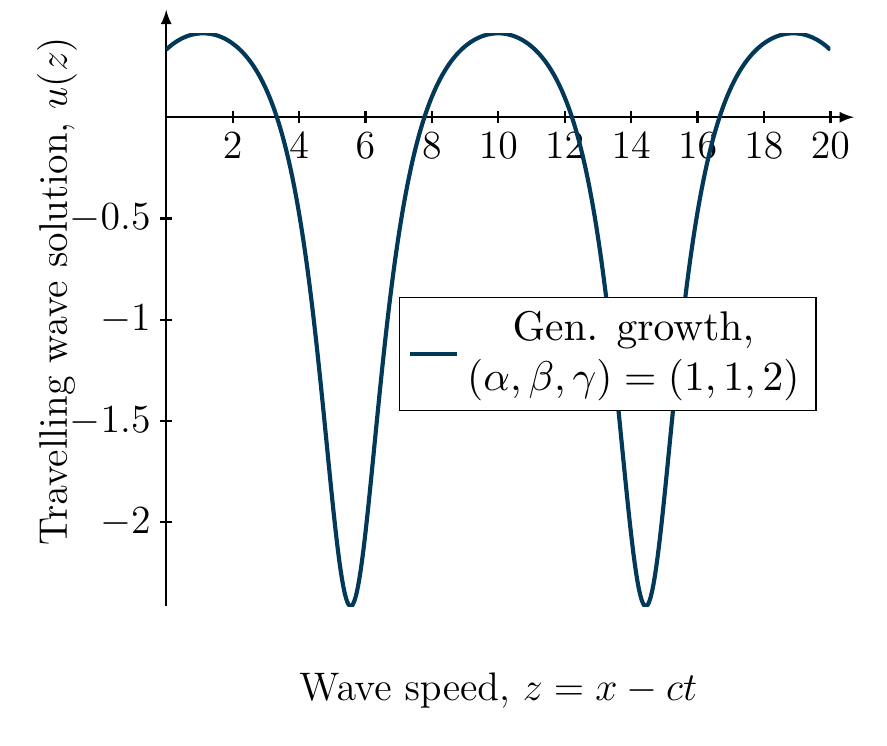
\begin{tikzpicture}
  % The axis of the plot
\begin{axis}[
    xlabel={Wave speed, $z=x-ct$},
    ylabel={Travelling wave solution, $u(z)$},
    x label style={at={(axis description cs:0.5,-0.1)},anchor=north},
    y label style={at={(axis description cs:-0.12,0.55)},rotate=90,anchor=south},
    scaled x ticks = false,
    %xtick={-1,-0.5,...,2},    
    %ymax = 3.22,
    %xmax = 4.5,
    legend style={at={(axis description cs:0.35,0.44)},anchor=west,nodes={scale=1.5, transform shape},align=center},
    label style={font=\Large},
    tick label style={font=\Large},
    legend cell align={left},
    grid style=dashed,
]
\addplot[
color=clr_2,line width=1.5pt,
]
coordinates {%
(0.0,0.3333333333333333)
(0.04008016032064128,0.33948396647772866)
(0.08016032064128256,0.3453452807996867)
(0.12024048096192384,0.3509250374925247)
(0.16032064128256512,0.3562305718081289)
(0.2004008016032064,0.36126880966725444)
(0.24048096192384769,0.36604628332483685)
(0.280561122244489,0.3705691461232601)
(0.32064128256513025,0.3748431863658922)
(0.3607214428857715,0.3788738403423503)
(0.4008016032064128,0.3826662045359348)
(0.4408817635270541,0.3862250470425259)
(0.48096192384769537,0.3895548182289639)
(0.5210420841683366,0.39265966065760594)
(0.561122244488978,0.3955434183023409)
(0.6012024048096192,0.39820964507990453)
(0.6412825651302605,0.40066161271885786)
(0.6813627254509018,0.40290231798709897)
(0.721442885771543,0.4049344892972726)
(0.7615230460921844,0.40676059270793213)
(0.8016032064128256,0.40838283733680136)
(0.8416833667334669,0.40980318020098194)
(0.8817635270541082,0.41102333049745615)
(0.9218436873747494,0.4120447533357503)
(0.9619238476953907,0.4128686729331499)
(1.002004008016032,0.41349607528139093)
(1.0420841683366733,0.413927710292301)
(1.0821643286573146,0.4141640934284118)
(1.122244488977956,0.41420550682313384)
(1.1623246492985972,0.4140519998936466)
(1.2024048096192383,0.413703389448234)
(1.2424849699398797,0.41315925928836417)
(1.282565130260521,0.41241895930439715)
(1.3226452905811623,0.4114816040623657)
(1.3627254509018036,0.41034607087785746)
(1.4028056112224447,0.4090109973715791)
(1.442885771543086,0.40747477849975167)
(1.4829659318637274,0.405735563051028)
(1.5230460921843687,0.403791249600166)
(1.56312625250501,0.40163948190722093)
(1.6032064128256511,0.39927764374953806)
(1.6432865731462925,0.3967028531723379)
(1.6833667334669338,0.3939119561421843)
(1.723446893787575,0.39090151958612296)
(1.7635270541082164,0.38766782379776565)
(1.8036072144288577,0.3842068541900915)
(1.8436873747494988,0.3805142923732331)
(1.8837675350701402,0.37658550653403117)
(1.9238476953907815,0.37241554109268404)
(1.9639278557114228,0.36799910561039223)
(2.004008016032064,0.3633305629205319)
(2.0440881763527052,0.35840391645459496)
(2.0841683366733466,0.35321279673292677)
(2.124248496993988,0.34775044698921564)
(2.164328657314629,0.3420097078967623)
(2.2044088176352705,0.3359830013638225)
(2.244488977955912,0.32966231336482754)
(2.284569138276553,0.32303917577409275)
(2.3246492985971945,0.316104647168785)
(2.3647294589178354,0.30884929256852706)
(2.4048096192384767,0.3012631620801443)
(2.444889779559118,0.2933357684178244)
(2.4849699398797593,0.2850560632714782)
(2.5250501002004007,0.2764124124995147)
(2.565130260521042,0.26739257012673295)
(2.6052104208416833,0.2579836511337921)
(2.6452905811623246,0.24817210303197532)
(2.685370741482966,0.23794367622597432)
(2.7254509018036073,0.2272833931785053)
(2.7655310621242486,0.21617551640406957)
(2.8056112224448895,0.20460351533551357)
(2.845691382765531,0.19255003212669378)
(2.885771543086172,0.17999684647805986)
(2.9258517034068134,0.16692483959996765)
(2.9659318637274548,0.15331395746173263)
(3.006012024048096,0.13914317351368427)
(3.0460921843687374,0.12439045111569873)
(3.0861723446893787,0.10903270595996979)
(3.12625250501002,0.09304576883934844)
(3.1663326653306614,0.07640434918680178)
(3.2064128256513023,0.059081999898017865)
(3.2464929859719436,0.04105108404961443)
(3.286573146292585,0.022282744241822736)
(3.3266533066132262,0.0027468754290135952)
(3.3667334669338675,-0.017587897743497463)
(3.406813627254509,-0.03875423789974575)
(3.44689378757515,-0.06078610478967563)
(3.4869739478957915,-0.08371875640788125)
(3.527054108216433,-0.10758873947496289)
(3.567134268537074,-0.13243386708088423)
(3.6072144288577155,-0.15829318094986441)
(3.6472945891783564,-0.18520689540443203)
(3.6873747494989977,-0.21321631967954224)
(3.727454909819639,-0.24236375476372723)
(3.7675350701402803,-0.27269236042184647)
(3.8076152304609217,-0.3042459874829552)
(3.847695390781563,-0.33706896985911317)
(3.8877755511022043,-0.3712058701009895)
(3.9278557114228456,-0.40670117160198027)
(3.967935871743487,-0.4435989098468225)
(4.008016032064128,-0.48194223438195133)
(4.04809619238477,-0.5217728924892989)
(4.0881763527054105,-0.5631306249082639)
(4.128256513026052,-0.6060524634194117)
(4.168336673346693,-0.6505719197385955)
(4.208416833667335,-0.6967180550489874)
(4.248496993987976,-0.7445144197162069)
(4.288577154308617,-0.7939778534049707)
(4.328657314629258,-0.8451171370826999)
(4.368737474949899,-0.8979314904175296)
(4.408817635270541,-0.9524089110372431)
(4.448897795591182,-1.008524356210919)
(4.488977955911824,-1.0662377729552273)
(4.529058116232465,-1.1254919895570257)
(4.569138276553106,-1.1862104902265822)
(4.609218436873747,-1.2482951051853877)
(4.649298597194389,-1.3116236610012184)
(4.68937875751503,-1.376047650336174)
(4.729458917835671,-1.441389996220283)
(4.7695390781563125,-1.5074430030203638)
(4.809619238476953,-1.5739666036699604)
(4.849699398797595,-1.6406870293537332)
(4.889779559118236,-1.7072960422262018)
(4.929859719438878,-1.7734508820577943)
(4.969939879759519,-1.8387750818015016)
(5.01002004008016,-1.9028603026375497)
(5.050100200400801,-1.9652693237701135)
(5.090180360721443,-2.0255402941054115)
(5.130260521042084,-2.08319231057118)
(5.170340681362725,-2.1377323309324945)
(5.210420841683367,-2.18866335865079)
(5.2505010020040075,-2.235493756511761)
(5.290581162324649,-2.277747459207428)
(5.33066132264529,-2.314974769391009)
(5.370741482965932,-2.346763344903637)
(5.410821643286573,-2.372748925501474)
(5.4509018036072145,-2.392625313688612)
(5.490981963927855,-2.4061531227871393)
(5.531062124248497,-2.4131668399966344)
(5.571142284569138,-2.413579823094508)
(5.611222444889779,-2.4073869526896114)
(5.651302605210421,-2.3946647897179583)
(5.691382765531062,-2.375569229196887)
(5.731462925851703,-2.3503307833978155)
(5.771543086172344,-2.319247757715574)
(5.811623246492986,-2.282677689336066)
(5.851703406813627,-2.2410274940414703)
(5.891783567134269,-2.194742805713407)
(5.9318637274549095,-2.1442969959838014)
(5.971943887775551,-2.0901803314706826)
(6.012024048096192,-2.032889669440341)
(6.052104208416833,-1.9729190176230824)
(6.092184368737475,-1.9107511988907568)
(6.132264529058116,-1.8468507746790157)
(6.1723446893787575,-1.7816582992013326)
(6.212424849699398,-1.7155859046851607)
(6.25250501002004,-1.649014159187109)
(6.292585170340681,-1.582290094351461)
(6.332665330661323,-1.515726270612767)
(6.372745490981964,-1.4496007305550176)
(6.4128256513026045,-1.3841576854729547)
(6.452905811623246,-1.3196087833450882)
(6.492985971943887,-1.2561348160873884)
(6.533066132264529,-1.1938877379419401)
(6.57314629258517,-1.1329928832907)
(6.613226452905812,-1.0735512895523982)
(6.6533066132264524,-1.0156420479687618)
(6.693386773547094,-0.9593246212033373)
(6.733466933867735,-0.9046410812462685)
(6.773547094188377,-0.8516182338643036)
(6.813627254509018,-0.8002696066639423)
(6.853707414829659,-0.7505972867851852)
(6.8937875751503,-0.7025936014402632)
(6.933867735470941,-0.6562426401341774)
(6.973947895791583,-0.6115216216556477)
(7.014028056112224,-0.5684021120168087)
(7.054108216432866,-0.5268511016485627)
(7.0941883767535066,-0.48683195151057296)
(7.134268537074148,-0.4483052185141147)
(7.174348697394789,-0.41122937092388223)
(7.214428857715431,-0.37556140432020235)
(7.254509018036072,-0.34125736836418585)
(7.294589178356713,-0.30827281409422264)
(7.3346693386773545,-0.27656317085572774)
(7.374749498997995,-0.24608406127556465)
(7.414829659318637,-0.21679156197518187)
(7.454909819639278,-0.18864241699923773)
(7.49498997995992,-0.1615942102388253)
(7.535070140280561,-0.13560550246369116)
(7.575150300601202,-0.11063593795452148)
(7.615230460921843,-0.08664632514940279)
(7.655310621242485,-0.06359869519000194)
(7.695390781563126,-0.04145634177312964)
(7.735470941883767,-0.02018384528079448)
(7.775551102204409,0.00025291622543739727)
(7.8156312625250495,0.01988676690495971)
(7.855711422845691,0.038749241998374234)
(7.895791583166332,0.05687060398207135)
(7.935871743486974,0.07427986458885498)
(7.975951903807615,0.09100481147396704)
(8.016032064128256,0.10707203848717223)
(8.056112224448897,0.12250697866933428)
(8.09619238476954,0.13733393922886952)
(8.13627254509018,0.1515761378720049)
(8.176352705410821,0.1652557399630791)
(8.216432865731463,0.1783938960792337)
(8.256513026052104,0.1910107795995259)
(8.296593186372744,0.2031256240332973)
(8.336673346693386,0.21475675984800374)
(8.376753507014028,0.22592165060388628)
(8.41683366733467,0.23663692824291613)
(8.45691382765531,0.24691842741336312)
(8.496993987975952,0.2567812187399348)
(8.537074148296593,0.26623964097346664)
(8.577154308617233,0.2753073319742572)
(8.617234468937875,0.28399725849984697)
(8.657314629258517,0.29232174478189327)
(8.697394789579159,0.3002924998881456)
(8.737474949899799,0.3079206438747886)
(8.77755511022044,0.31521673274186657)
(8.817635270541082,0.32219078221044317)
(8.857715430861724,0.3288522903447891)
(8.897795591182364,0.33521025904642976)
(8.937875751503006,0.3412732144495144)
(8.977955911823647,0.34704922624881446)
(9.018036072144287,0.3525459259928714)
(9.05811623246493,0.35777052437546303)
(9.098196392785571,0.3627298275587857)
(9.138276553106213,0.3674302525615871)
(9.178356713426853,0.3718778417450328)
(9.218436873747494,0.37607827642837977)
(9.258517034068136,0.38003688966562754)
(9.298597194388778,0.3837586782132617)
(9.338677354709418,0.3872483137180021)
(9.37875751503006,0.39051015315219356)
(9.418837675350701,0.39354824852310777)
(9.458917835671341,0.3963663558810157)
(9.498997995991983,0.39896794364942617)
(9.539078156312625,0.40135620029941016)
(9.579158316633267,0.403534041388429)
(9.619238476953907,0.40550411598257763)
(9.659318637274549,0.4072688124796448)
(9.69939879759519,0.408830263848887)
(9.739478957915832,0.4101903523019102)
(9.779559118236472,0.41135071340756524)
(9.819639278557114,0.4123127396622763)
(9.859719438877756,0.4130775835257525)
(9.899799599198396,0.4136461599305727)
(9.939879759519037,0.4140191482726767)
(9.97995991983968,0.4141969938883592)
(10.02004008016032,0.4141799090219197)
(10.06012024048096,0.41396787328669954)
(10.100200400801603,0.4135606336208007)
(10.140280561122244,0.41295770373736684)
(10.180360721442886,0.41215836306787185)
(10.220440881763526,0.41116165519544307)
(10.260521042084168,0.4099663857738075)
(10.30060120240481,0.4085711199260184)
(10.34068136272545,0.4069741791156694)
(10.380761523046091,0.4051736374818547)
(10.420841683366733,0.40316731762766705)
(10.460921843687375,0.4009527858505536)
(10.501002004008015,0.3985273468013647)
(10.541082164328657,0.39588803755743657)
(10.581162324649299,0.39303162109355233)
(10.62124248496994,0.3899545791331081)
(10.66132264529058,0.38665310436031425)
(10.701402805611222,0.3831230919727461)
(10.741482965931864,0.37936013055206863)
(10.781563126252504,0.3753594922292732)
(10.821643286573146,0.37111612211932504)
(10.861723446893787,0.36662462699870135)
(10.901803607214429,0.36187926319796004)
(10.941883767535069,0.35687392368019855)
(10.98196392785571,0.3516021242751014)
(11.022044088176353,0.34605698903723336)
(11.062124248496994,0.3402312346963604)
(11.102204408817634,0.33411715416692084)
(11.142284569138276,0.32770659908335886)
(11.182364729458918,0.3209909613279375)
(11.222444889779558,0.31396115351793064)
(11.2625250501002,0.3066075884198579)
(11.302605210420841,0.29892015725971904)
(11.342685370741483,0.29088820690017253)
(11.382765531062123,0.2825005158583713)
(11.422845691382765,0.27374526914189207)
(11.462925851703407,0.2646100318850557)
(11.503006012024048,0.25508172177410066)
(11.543086172344688,0.24514658025743058)
(11.58316633266533,0.23479014254676644)
(11.623246492985972,0.2239972064267859)
(11.663326653306612,0.21275179990515375)
(11.703406813627254,0.20103714775212375)
(11.743486973947896,0.18883563699964176)
(11.783567134268537,0.1761287814946631)
(11.823647294589177,0.16289718563088312)
(11.863727454909819,0.14912050741798194)
(11.90380761523046,0.13477742108876095)
(11.943887775551103,0.11984557949302056)
(11.983967935871743,0.10430157658398809)
(12.024048096192384,0.08812091036972518)
(12.064128256513026,0.0712779467796507)
(12.104208416833666,0.05374588498679642)
(12.144288577154308,0.03549672483142764)
(12.18436873747495,0.016501237113254658)
(12.224448897795591,-0.003271062340123097)
(12.264529058116231,-0.023851933759175478)
(12.304609218436873,-0.04527442841777746)
(12.344689378757515,-0.06757289605023256)
(12.384769539078157,-0.09078298298978904)
(12.424849699398797,-0.11494161904260292)
(12.464929859719438,-0.14008699079874162)
(12.50501002004008,-0.16625849872970144)
(12.54509018036072,-0.19349669502681394)
(12.585170340681362,-0.22184319869422858)
(12.625250501002004,-0.251340583921784)
(12.665330661322646,-0.2820322372259922)
(12.705410821643286,-0.3139621782620111)
(12.745490981963927,-0.3471748385785256)
(12.785571142284569,-0.3817147919161119)
(12.825651302605209,-0.41762642894757657)
(12.86573146292585,-0.4549535686398266)
(12.905811623246493,-0.49373899770183133)
(12.945891783567134,-0.5340239289012387)
(12.985971943887774,-0.5758473684212903)
(13.026052104208416,-0.619245381941459)
(13.066132264529058,-0.664250248824589)
(13.1062124248497,-0.7108894937628567)
(13.14629258517034,-0.7591847855761081)
(13.186372745490981,-0.8091506936920614)
(13.226452905811623,-0.8607932943134038)
(13.266533066132263,-0.9141086205602448)
(13.306613226452905,-0.969080954154871)
(13.346693386773547,-1.0256809606925286)
(13.386773547094188,-1.0838636764264846)
(13.426853707414828,-1.1435663619876366)
(13.46693386773547,-1.2047062477310078)
(13.507014028056112,-1.2671782065664716)
(13.547094188376754,-1.3308524032080835)
(13.587174348697394,-1.3955719836436697)
(13.627254509018035,-1.4611508849693198)
(13.667334669338677,-1.527371862987596)
(13.707414829659317,-1.593984852266562)
(13.747494989979959,-1.660705789483072)
(13.7875751503006,-1.7272160442455233)
(13.827655310621243,-1.7931626102760008)
(13.867735470941883,-1.8581592116178018)
(13.907815631262524,-1.9217884710781943)
(13.947895791583166,-1.9836052691619868)
(13.987975951903808,-2.0431413894405672)
(14.028056112224448,-2.099911499543146)
(14.06813627254509,-2.1534204558351346)
(14.108216432865731,-2.2031718459956577)
(14.148296593186371,-2.2486776005786133)
(14.188376753507013,-2.2894684175970683)
(14.228456913827655,-2.3251046602760193)
(14.268537074148297,-2.355187315629223)
(14.308617234468937,-2.3793685490309127)
(14.348697394789578,-2.397361365320475)
(14.38877755511022,-2.408947896086327)
(14.428857715430862,-2.4139858784486448)
(14.468937875751502,-2.412412971872226)
(14.509018036072144,-2.404248671147006)
(14.549098196392785,-2.3895937067795265)
(14.589178356713425,-2.368626966987135)
(14.629258517034067,-2.341600115329321)
(14.669338677354709,-2.308830202208295)
(14.70941883767535,-2.2706906665210322)
(14.74949899799599,-2.227601188449699)
(14.789579158316633,-2.1800168825442126)
(14.829659318637274,-2.128417312753156)
(14.869739478957916,-2.073295772301365)
(14.909819639278556,-2.0151492082639018)
(14.949899799599198,-1.954469091699334)
(14.98997995991984,-1.8917334478404189)
(15.03006012024048,-1.8274001748731714)
(15.070140280561121,-1.7619017005649749)
(15.110220440881763,-1.6956409578881517)
(15.150300601202405,-1.6289886063921297)
(15.190380761523045,-1.5622813862597953)
(15.230460921843687,-1.4958214662154437)
(15.270541082164328,-1.4298766332285837)
(15.31062124248497,-1.364681169188955)
(15.35070140280561,-1.300437265082697)
(15.390781563126252,-1.2373168343737013)
(15.430861723446894,-1.1754636021965266)
(15.470941883767534,-1.1149953638252241)
(15.511022044088175,-1.0560063232892565)
(15.551102204408817,-0.9985694399172097)
(15.591182364729459,-0.942738726283712)
(15.631262525050099,-0.888551455077508)
(15.67134268537074,-0.8360302445817795)
(15.711422845691382,-0.785185002713728)
(15.751503006012024,-0.736014717977665)
(15.791583166332664,-0.688509092389894)
(15.831663326653306,-0.6426500166227366)
(15.871743486973948,-0.5984128914964028)
(15.911823647294588,-0.5557678027280012)
(15.95190380761523,-0.5146805577241059)
(15.991983967935871,-0.4751135943553063)
(16.03206412825651,-0.43702677223491565)
(16.072144288577153,-0.4003780571747693)
(16.112224448897795,-0.3651241093206065)
(16.152304609218437,-0.3312207850704336)
(16.19238476953908,-0.2986235623256679)
(16.23246492985972,-0.26728789797449415)
(16.27254509018036,-0.23716952580498488)
(16.312625250501,-0.20822470232571666)
(16.352705410821642,-0.18041040725848576)
(16.392785571142284,-0.1536845047787776)
(16.432865731462925,-0.1280058709266978)
(16.472945891783567,-0.10333449200122707)
(16.51302605210421,-0.07963153818816325)
(16.55310621242485,-0.056859416158167614)
(16.59318637274549,-0.03498180390587895)
(16.63326653306613,-0.013963670682303794)
(16.673346693386772,0.006228715501524336)
(16.713426853707414,0.02562779065455347)
(16.753507014028056,0.0442647060188101)
(16.793587174348698,0.062169346124637065)
(16.83366733466934,0.07937035232506809)
(16.873747494989978,0.09589515064572388)
(16.91382765531062,0.11176998296060736)
(16.95390781563126,0.12701994065539374)
(16.993987975951903,0.14166900007102254)
(17.034068136272545,0.1557400591338287)
(17.074148296593187,0.16925497467629738)
(17.11422845691383,0.18223460003675168)
(17.154308617234467,0.1946988225985091)
(17.19438877755511,0.20666660099091494)
(17.23446893787575,0.21815600172739769)
(17.274549098196392,0.2291842351006768)
(17.314629258517034,0.23976769019332173)
(17.354709418837675,0.24992196889412097)
(17.394789579158317,0.25966191883788015)
(17.43486973947896,0.26900166520904056)
(17.474949899799597,0.27795464136855774)
(17.51503006012024,0.2865336182792985)
(17.55511022044088,0.29475073271822316)
(17.595190380761522,0.3026175142743842)
(17.635270541082164,0.3101449111403881)
(17.675350701402806,0.317343314711979)
(17.715430861723448,0.3242225830159207)
(17.755511022044086,0.3307920629906251)
(17.795591182364728,0.3370606116472505)
(17.83567134268537,0.3430366161413526)
(17.87575150300601,0.34872801278682736)
(17.915831663326653,0.3541423050449109)
(17.955911823647295,0.35928658052151696)
(17.995991983967937,0.36416752700629645)
(18.036072144288575,0.36879144758654697)
(18.076152304609217,0.37316427486856935)
(18.11623246492986,0.3772915843382849)
(18.1563126252505,0.38117860689199184)
(18.196392785571142,0.38483024056701837)
(18.236472945891784,0.38825106150081495)
(18.276553106212425,0.3914453341457217)
(18.316633266533067,0.3944170207652565)
(18.356713426853705,0.3971697902363504)
(18.396793587174347,0.3997070261804869)
(18.43687374749499,0.4020318344452091)
(18.47695390781563,0.40414704995596945)
(18.517034068136272,0.4060552429567745)
(18.557114228456914,0.40775872465657376)
(18.597194388777556,0.40925955229684385)
(18.637274549098194,0.4105595336543073)
(18.677354709418836,0.41166023099124815)
(18.717434869739478,0.4125629644644016)
(18.75751503006012,0.4132688150019284)
(18.79759519038076,0.41377862665652454)
(18.837675350701403,0.41409300844126923)
(18.877755511022045,0.4142123356533714)
(18.917835671342683,0.4141367506895439)
(18.957915831663325,0.41386616335530074)
(18.997995991983966,0.4134002506690523)
(19.03807615230461,0.4127384561604432)
(19.07815631262525,0.4118799886609584)
(19.118236472945892,0.4108238205833876)
(19.158316633266534,0.4095686856853125)
(19.198396793587175,0.4081130763103358)
(19.238476953907814,0.40645524009932915)
(19.278557114228455,0.4045931761625149)
(19.318637274549097,0.4025246307017384)
(19.35871743486974,0.4002470920707999)
(19.39879759519038,0.39775778526023897)
(19.438877755511022,0.39505366579146234)
(19.478957915831664,0.3921314130036005)
(19.519038076152302,0.38898742271497894)
(19.559118236472944,0.38561779923957057)
(19.599198396793586,0.3820183467372996)
(19.639278557114228,0.3781845598755715)
(19.67935871743487,0.3741116137779314)
(19.71943887775551,0.36979435323431925)
(19.759519038076153,0.36522728114599223)
(19.79959919839679,0.360404546176862)
(19.839679358717433,0.3553199295817414)
(19.879759519038075,0.34996683118087935)
(19.919839679358716,0.3443382544491508)
(19.95991983967936,0.33842679068746684)
(20.0,0.33222460224337624)
};
\addlegendentry{Gen. growth,\\ $(\alpha,\beta,\gamma)=(1,1,2)$}

\end{axis}
\end{tikzpicture}
%=========================================================================================================
\end{document}
